\section*{Introduction}


\section{Le matériel}



\section{Théorie}
\subsection{Quelques équations}


\begin{equation*}
    \begin{pmatrix}
        p_{out}\\
        u_{out}
    \end{pmatrix}
    =
    \begin{pmatrix}
        \cos{kL} & -iZ_c\sin{kL}\\
        -\frac{i}{Z_c}\sin{kL} & \cos{kL}
    \end{pmatrix}
    \begin{pmatrix}
        p_{in}\\
        u_{in}
    \end{pmatrix}
\end{equation*}

Avec $Z_c$ l'impédance caractéristique du milieu de propagation, ici de l'air à température ambiante. Soit $Zc=\rho_0 c_0$, $k$ le nombre d'onde de l'onde propagée, ici $k=\omega/c_0$ avec $\omega$ la pulsation de l'onde et D la section du tube. 



\subsection{Le diaphragme}

\subsubsection{Régime linéaire}

\begin{equation*}
    Z_{in}=-\frac{Z_c\tan kL + \frac{1-\alpha}{2}}{\frac{1-\alpha}{2Z_c}\tan kL+1}
\end{equation*}

\subsubsection{Régime non linéaire}

\begin{equation*}
    Z_{NL}=\frac{d\tilde{p}}{\tilde{v}_0}=1.2\rho_0K(v_0)_{RMS}
\end{equation*}

\section{Expérimentations}
\subsection{Montage expérimental}

\begin{figure}[!ht]
				\centering
				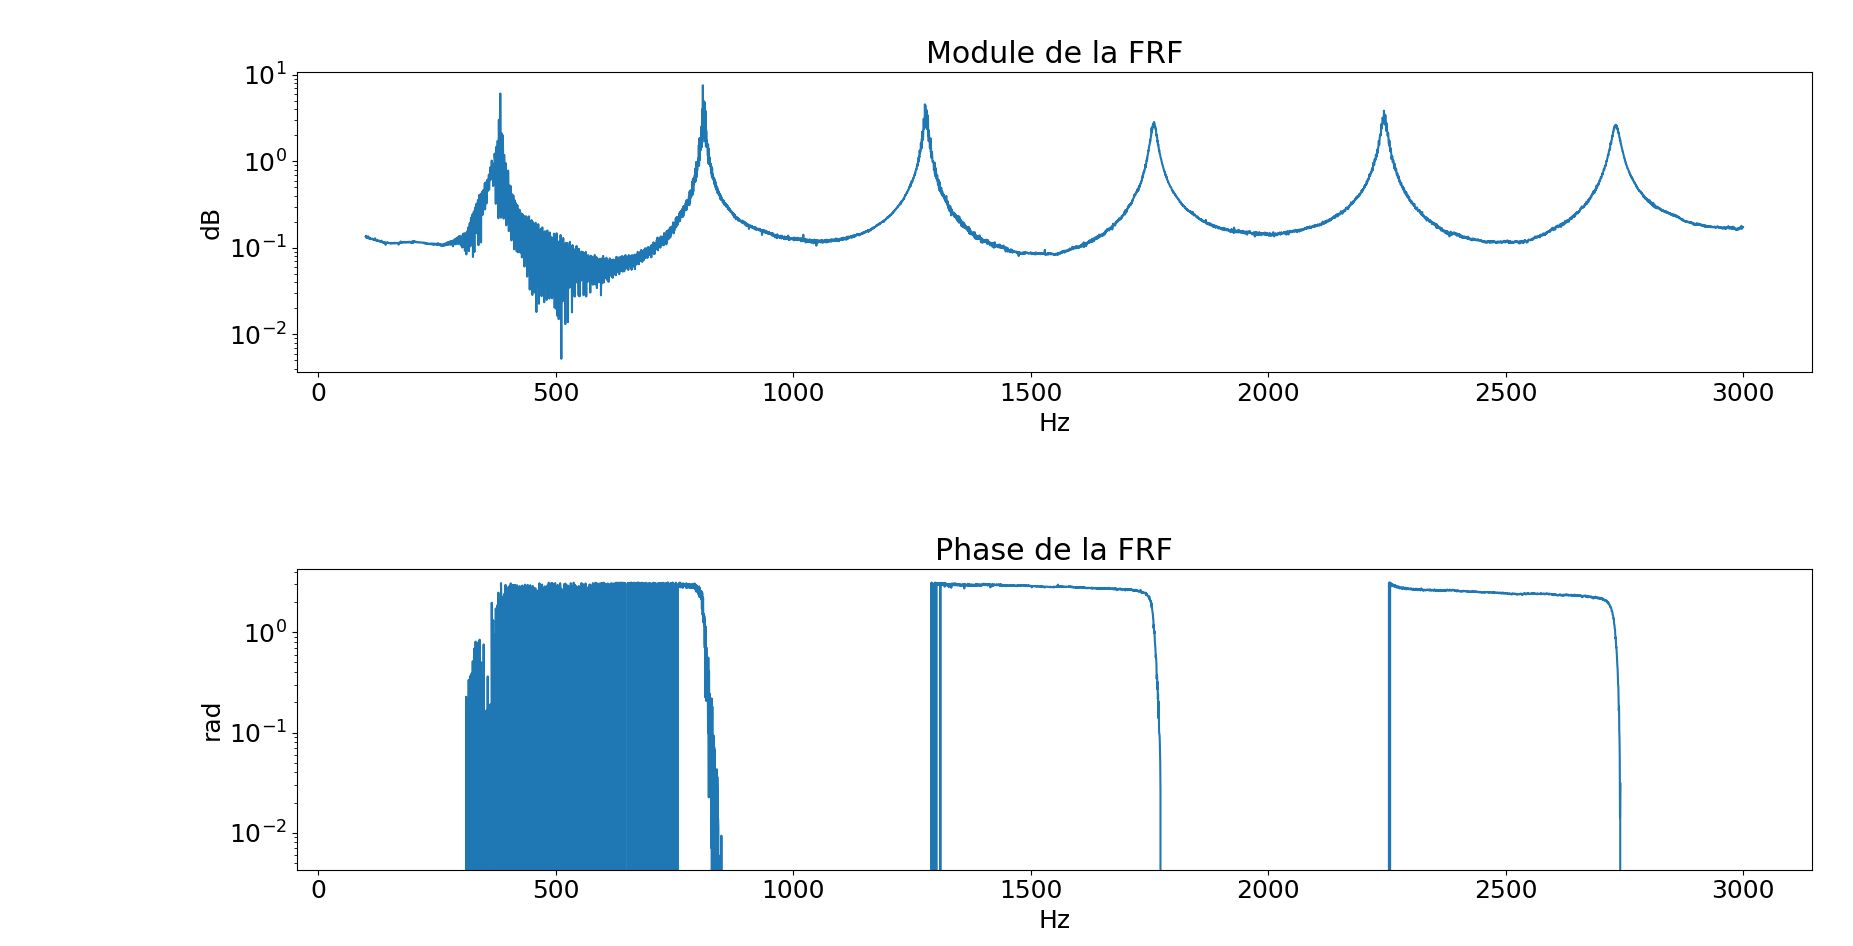
\includegraphics[scale=0.3, clip]{pics/frf_0007_ferme.png}
				\caption{Fonction de transfert avec le diaphragme en régime linéaire}
				\label{ferme}
\end{figure}


\newpage
\subsection{Mesures en régime non linéaire}


\section{Code et implémentation}

Cette section présente le code utilisé pour l'analyse des données et les calculs théoriques.

\subsection{Exemple de traitement des données en Python}

Le code suivant montre un exemple d'analyse spectrale d'un signal sinusoïdal discrétisé :

\begin{lstlisting}[language=Python, caption=Analyse spectrale d'un signal sinusoïdal]
import numpy as np
import matplotlib.pyplot as plt
from scipy import signal

# Paramètres du signal
fs = 1000  # Fréquence d'échantillonnage (Hz)
f_signal = 50  # Fréquence du signal (Hz)
t_duration = 2  # Durée du signal (s)

# Génération du vecteur temps
t = np.linspace(0, t_duration, int(fs * t_duration), endpoint=False)

# Génération du signal sinusoïdal avec bruit
signal_clean = np.sin(2 * np.pi * f_signal * t)
noise = 0.1 * np.random.normal(size=t.shape)
signal_noisy = signal_clean + noise

# Calcul de la FFT
frequencies, power_spectrum = signal.welch(signal_noisy, fs, 
                                         nperseg=512, 
                                         scaling='density')

# Affichage des résultats
plt.figure(figsize=(12, 8))

# Signal temporel
plt.subplot(2, 1, 1)
plt.plot(t[:500], signal_noisy[:500], 'b-', linewidth=0.8)
plt.plot(t[:500], signal_clean[:500], 'r--', linewidth=1.5)
plt.xlabel('Temps (s)')
plt.ylabel('Amplitude')
plt.title('Signal temporel')
plt.legend(['Signal bruité', 'Signal théorique'])
plt.grid(True, alpha=0.3)

# Spectre fréquentiel
plt.subplot(2, 1, 2)
plt.semilogy(frequencies, power_spectrum)
plt.xlabel('Fréquence (Hz)')
plt.ylabel('Densité spectrale de puissance')
plt.title('Analyse spectrale')
plt.grid(True, alpha=0.3)
plt.xlim(0, 100)

plt.tight_layout()
plt.show()

# Calcul de l'impédance caractéristique
rho_0 = 1.225  # Densité de l'air (kg/m³)
c_0 = 343      # Vitesse du son (m/s)
Z_c = rho_0 * c_0

print(f"Impédance caractéristique de l'air : {Z_c:.1f} Pa.s/m³")
\end{lstlisting}

\subsection{Fonctions utilitaires}

Voici quelques fonctions utiles pour les calculs d'acoustique :

\begin{lstlisting}[language=Python, caption=Fonctions pour les calculs acoustiques]
def calculate_wavelength(frequency, sound_speed=343):
    """
    Calcule la longueur d'onde d'un signal acoustique.
    
    Args:
        frequency: Fréquence en Hz
        sound_speed: Vitesse du son en m/s (défaut: 343 m/s)
    
    Returns:
        Longueur d'onde en mètres
    """
    return sound_speed / frequency

def pressure_to_db(pressure, reference=20e-6):
    """
    Convertit une pression acoustique en décibels SPL.
    
    Args:
        pressure: Pression acoustique en Pa
        reference: Pression de référence (défaut: 20 µPa)
    
    Returns:
        Niveau sonore en dB SPL
    """
    return 20 * np.log10(np.abs(pressure) / reference)

# Exemple d'utilisation
freq = 1000  # Hz
wavelength = calculate_wavelength(freq)
pressure = 0.02  # Pa
db_level = pressure_to_db(pressure)

print(f"Fréquence: {freq} Hz")
print(f"Longueur d'onde: {wavelength:.3f} m")
print(f"Niveau sonore: {db_level:.1f} dB SPL")
\end{lstlisting}


\section*{Conclusion}

\section*{Digression}
